%----------------------------------------------------------------------------------------
%	PACKAGES AND DOCUMENT CONFIGURATIONS
%----------------------------------------------------------------------------------------
\documentclass[article, a4paper, 11pt, oneside]{memoir}

% Margins
\usepackage[top=3cm,left=2cm,right=2cm,bottom=3cm]{geometry}

% Encondings
\usepackage[utf8]{inputenc}

% Language
\usepackage[portuguese]{babel}

% Graphics and images
\usepackage{graphicx}
	\graphicspath{{../images/}}

% Tables
\usepackage{tabularx}

% Paragraph Spacing
\usepackage{parskip}
\usepackage{indentfirst}
\setlength{\parskip}{0.4cm}

% Hyperreferences
\usepackage{hyperref}

% Repeated commands
\usepackage{expl3}
\ExplSyntaxOn
\cs_new_eq:NN \Repeat \prg_replicate:nn
\ExplSyntaxOff

% Header and Footer Things
\usepackage{wallpaper}
\usepackage{fancyhdr}

% Following code to edit the pagestyle
\pagestyle{fancy}
\fancyhf{}
\rhead{RCOM}
\rfoot{Página \thepage}

% Commands
\usepackage{xargs}

%% Linked Email
\newcommand{\email}[1]{
{\texttt{\href{mailto:#1}{#1}} }
}

% Code
\usepackage{listings}
\lstset{language=C}
\usepackage{color}
\definecolor{dkgreen}{rgb}{0,0.6,0}
\definecolor{gray}{rgb}{0.5,0.5,0.5}
\definecolor{mauve}{rgb}{0.58,0,0.82}

\lstset{frame=tb,
  language=C,
  aboveskip=3mm,
  belowskip=3mm,
  showstringspaces=false,
  columns=flexible,
  basicstyle={\small\ttfamily},
  numbers=none,
  numberstyle=\tiny\color{gray},
  keywordstyle=\color{blue},
  commentstyle=\color{dkgreen},
  stringstyle=\color{mauve},
  breaklines=true,
  breakatwhitespace=true,
  tabsize=3
}

%----------------------------------------------------------------------------------------
%	DOCUMENT INFORMATION
%----------------------------------------------------------------------------------------
% Title
\title{\Huge \texttt{Relatório do 1º Trabalho Laboratorial} }
% Authors
\author{
\LARGE \textbf{Grupo 5}\\\\
\begin{tabular}{l r}
	\email{up201806551@fe.up.pt} & Beatriz Costa Silva Mendes			\\
	\email{up201806528@fe.up.pt} & Clara Alves Martins		            \\
\end{tabular}
}


%\institute{Faculdade de Engenharia da Universidade do Porto - RCOM}

% Date for the report
\date{\today}

% Table of Contents
\addto\captionsportuguese{\renewcommand*\contentsname{Índice}}

%----------------------------------------------------------------------------------------
%	DOCUMENT
%----------------------------------------------------------------------------------------
\begin{document}
%----------------------------------------------------------------------------------------
%	Front Page
%----------------------------------------------------------------------------------------
% Title Author and Date
\maketitle

% More information for front page
\begin{center}
\textbf{Redes de Computadores - 2020/21 - MIEIC}
\Repeat{2}{\linebreak}
\begin{tabular}{l r}
	\textbf{Professor das Aulas Laboratoriais}: & Manuel Alberto Pereira Ricardo
\end{tabular}
\Repeat{4}{\linebreak}
% FEUP Logo

\includegraphics[scale=0.4]{img/FEUPlogo.png}

\end{center}

\newpage
% Header Image
\CenterWallPaper{0.1}{img/FEUPlogo.png}
\addtolength{\wpXoffset}{-7.5cm}
\addtolength{\wpYoffset}{13.8cm}

%----------------------------------------------------------------------------------------
%	TABLE OF CONTENTS
%----------------------------------------------------------------------------------------
\tableofcontents*


\subsection{Sumário}

Este relatório tem como objetivo resumir todo o trabalho que foi realizado ao longo das
aulas práticas. Este consite na criação de uma aplicação que auxilia na transferência de
ficheiros através de uma porta de série, tendo-se, assim, criado diversas funções e estruturas
de dados que tornam esta transferência possível.

Após vários testes realizados em casa através do comando fornecido de \verb|socat|:

\begin{lstlisting}
  sudo socat -d  -d  PTY,link=/dev/ttyS0,mode=777   PTY,link=/dev/ttyS1,mode=777)
\end{lstlisting}

, através das portas série do laboratório (RS-232) e ainda portas série diferentes, concluimos
que o nosso programa transmite de maneira fiável um ficheiro de qualquer dimensão, mesmo quando
surgem erros, através de uma porta série.

%----------------------------------------------------------------------------------------
%	CHAPTER 1 - Introdução
%----------------------------------------------------------------------------------------
\chapter[Introdução][Introdução]{Introdução} \label{\thechapter}

O objetivo do trabalho que nos foi proposto é criar um protocolo de aplicação simples para 
realizar a transferência de um ficheiro, usando o serviço fiável oferecido pelo procolo de 
ligação de dados. Para estabelecer esta comunicação utilizamos as portas de série (portas de série 
RS-232 - comunicação assíncrona) que nos foram disponibilizadas ao longo das aulas práticas.
Todo o trabalho foi implementado de acordo com a informação que nos foi fornecida nos guiões
de trabalho. 

\begin{figure}[htbp]
    \centering        
    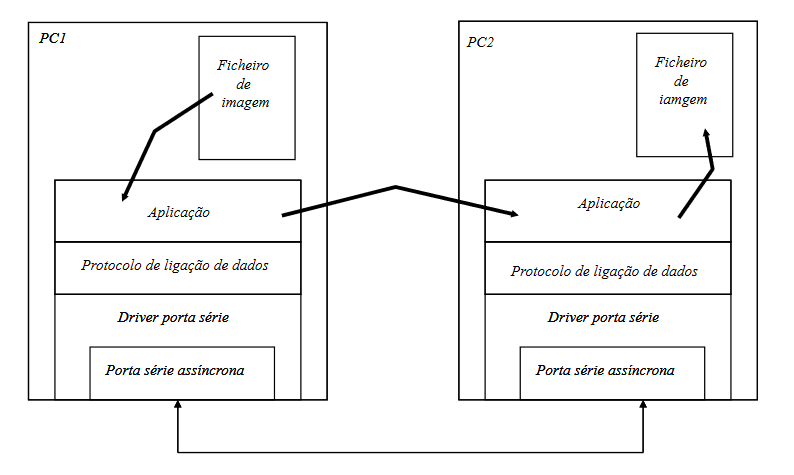
\includegraphics[scale=0.5]{img/aplicacao_teste.png}
    \caption{Aplicação Teste}
    \label{fig:Figura1}
\end{figure}

O relatório apresenta a seguinte estrutura:
\begin{enumerate}
    \item \textbf{Arquitetura}: blocos funcionais e interfaces da aplicação;
    \item \textbf{Estrutura do Código}: APIs, principais estruturas de dados, 
    principais funções e sua relação com a arquitetura;
    \item \textbf{Casos de Uso Principais}: identificação dos casos de uso principais
    e sequências de chamadas de funções;
    \item \textbf{Protocolo de Ligação Lógica}: identificação dos principais aspetos funcionais 
    e descrição da estratégia de implementação destes aspetos com apresentação de extratos de
    código;
    \item \textbf{Protocolo de Aplicação}: identificação dos principais aspetos funcionais 
    e descrição da estratégia de implementação destes aspetos com apresentação de extratos de
    código;
    \item \textbf{Validação}: descrição dos testes efectuados com apresentação quantificada 
    dos resultados;
    \item \textbf{Eficiência do Protocolo de Ligação de Dados}: caraterização estatística da 
    eficiência do protocolo, feita com recurso a medidas sobre o código desenvolvido;
    \item \textbf{Conclusões}: síntese da informação apresentada nas secções anteriores e 
    reflexão sobre os objectivos de aprendizagem alcançados.


\end{enumerate}

%----------------------------------------------------------------------------------------
%	CHAPTER 2 - Arquitetura
%----------------------------------------------------------------------------------------
\chapter[Arquitetura][Arquitetura]{Arquitetura} \label{\thechapter}

\section{Camadas}

O programa desenvolvido pelo nosso grupo de trabalho tem duas camadas muito bem definidas:
a \textbf{camada da aplicação} e a \textbf{camada da ligação de dados}.

A \textbf{camada da aplicação} é responsável pelo envio e receção de ficheiros. Relembrando
a Figura 1 presente na secção anterior, esta camada encontra-se acima da camada de ligação de
dados. Para além disso, esta ainda utiliza a interface disponibilizada pela camada de ligação
de dados, chamando as suas funções para auxiliar no envio e receção de ficheiros. A camada da aplicação 
foi desenvolvida nos ficheiros \verb|application_layer.c| e \verb|file_interaction.c|.

A \textbf{camada da ligação lógica}, por outro lado, tem como principal objetivo estabelecer
a ligação e assegurar a consistência do protocolo de ligação de dados que foi desenvolvido, sendo,
assim, a camada de mais baixo nível da aplicação. Esta camada realiza a interação com a porta de
série, fazendo a abertura, escrita, leitura e fecho desta, tratando ainda dos erros que poderão
surgir na transmissão através da técnica de \textit{byte stuffing}, garantindo assim a fiabilidade
na transmissão dos ficheiros. Esta camada foi desenvolvida no ficheiro \verb|logical_link.c|.

\section{Interface}

Na \textbf{interface} disponível para o utilizador, será apresentada informação relativamente
ao estado do envio e da receção do ficheiro, nomeadamente se o recetor e o transmissor estão
a ler ou a escrever tramas. Para além disso, também surgem mensagens de erro caso surja algum
durante a transmissão dos ficheiros.

%----------------------------------------------------------------------------------------
%	CHAPTER 3 - Estrutura do Código
%----------------------------------------------------------------------------------------
\chapter[Estrutura do Código][Estrutura do Código]{Estrutura do Código} \label{\thechapter}

Numa primeira fase, o nosso projeto tem dois ficheiros fundamentais: \verb|write.c| e \verb|read.c|.
Estes ficheiros são responsáveis por interligar a camada de ligação de dados e a camada da
aplicação de modo a que a transferência de ficheiros seja possível. Posteriormente,
os restantes ficheiros possuem funções e estruturas de dados que facilitam a transmissão, leitura
e escrita de tramas.

\section{Camada de Ligação de Dados}

\subsection{Estruturas de Dados:}
Criação de uma \textit{struct} \verb|packet| para armazenar os \textit{bytes} do pacote e o
tamanho deste.

Consultar Anexo II.

\subsection{Principais funções:}
Consultar Anexo III.

\subsection{Funções auxiliares:}
Consultar Anexo IV.

\section{Camada da Aplicação}

\subsection{Estruturas de Dados:}
Criação de duas \textit{structs}: \verb|control_packet| e \verb|data_packet|.
A primeira possui a informação necessária para utilizar um pacote de controlo e
a segunda para utilizar um pacote de informação.

Consultar Anexo V.

\subsection{Principais funções:}
Consultar Anexo VI.

\subsection{Funções auxiliares:}
Consultar Anexo VII.

%----------------------------------------------------------------------------------------
%	CHAPTER 4 - Casos de uso principais
%----------------------------------------------------------------------------------------
\chapter[Casos de Uso Principais][Casos de Uso Principais]{Casos de Uso Principais} \label{\thechapter}

\section{Transmissor (\textit{Transmitter})}

O programa é executado em modo \textbf{transmissor}. Inicialmente, verifica-se se o ficheiro que
se pretende transferir existe. Existindo, é estabelecida a ligação e, em seguida, vão sendo enviados pacotes
de dados de acordo com o protocolo de ligação implementado. Após a conclusão do envio, a ligação
é encerrada, terminando assim o programa. Em seguida apresenta-se a sequência de chamadas das 
funções principais:
\begin{enumerate}
    \item \verb|llopen|: abertura da porta de série para escrita e leitura, envio da trama SET e 
    receção da trama UA;
    \item \verb|construct_control_packet|: construção do pacote de controlo com a flag de início
    da transmissão e os restantes parâmetros;
    \item \verb|llwrite|: construção da trama que inclui o pacote de controlo, escrita deste e
    verificação de erros;
    \item Loop Principal:
    \begin{enumerate}
        \item \verb|read_from_file|: abertura do ficheiro que será transmitido e leitura deste;
        \item \verb|construct_data_packet|: construção do pacote de informação com base no lido
        do ficheiro aberto anteriormente;
        \item \verb|llwrite|: construção da trama que inclui o pacote de informação, escrita deste e
        verificação de erros;
    \end{enumerate}    
    \item \verb|construct_control_packet|: construção do pacote de controlo com a flag de início
    da transmissão e os restantes parâmetros;
    \item \verb|llwrite|: construção da trama que inclui o pacote de controlo, escrita deste e
    verificação de erros;
    \item \verb|llclose|: envio da trama DISC, receção da trama DISC, envio da trama UA
    e fecho da porta de série.
\end{enumerate}

\section{Recetor (\textit{Receiver})}

O programa é executado em modo \textbf{recetor}. É estabelecida a ligação com a porta de série.
Seguidamente, começam a ser lidos os pacotes enviados pelo trasnmissor. No final da leitura,
a ligação de dados é encerrada. Seguem-se as chamadas das funções principais por ordem de 
acontecimentos:
\begin{enumerate}
    \item \verb|llopen|: abertura da porta de série para escrita e leitura, receção da trama SET e 
    envio da trama UA;
    \item Loop Principal:
    \begin{enumerate}
        \item \verb|llread|: leitura das tramas que foram criadas pelo transmissor, quer sejam tramas com
        o pacote de controlo, quer sejam tramas com pacotes de informação, e verificação de erros;
        \begin{enumerate}
            \item Se for lido um pacote de informação:
            \begin{enumerate}
                \item \verb|deconstruct_data_packet|: desconstrução do pacote de informação que foi enviado
                pela ligação de dados;
                \item \verb|write_to_file|: escrita da informação recebida para o ficheiro;
            \end{enumerate}
            \item Se for lido um pacote de controlo:
            \begin{enumerate}
                \item \verb|deconstruct_control_packet|: desconstrução do pacote de controlo que foi enviado
                pela ligação de dados, verificando se é o do início ou do fim da transmissão;
            \end{enumerate}
        \end{enumerate}
    \end{enumerate}
    \item \verb|llclose|: envio da trama DISC, receção da trama UA e fecho da porta de série.
\end{enumerate}

%----------------------------------------------------------------------------------------
%	CHAPTER 5 - Protocolo de ligação lógica
%----------------------------------------------------------------------------------------
\chapter[Protocolo de Ligação Lógica][Protocolo de Ligação Lógica]{Protocolo de Ligação Lógica} \label{\thechapter}

\section{Aspetos Fundamentais e Estratégias de Implementação Adotadas}

\subsection{Estabelecimento/fecho da ligação lógica}
No caso do transmissor (\textit{transmitter}):

A ligação é estabelecida
através do envio de uma trama SET e receção de uma trama UA.

O fecho da ligação acontece quando é enviada uma trama DISC,
recebida uma trama DISC e enviada uma trama UA.

No caso do recetor (\textit{receiver}):

A ligação é estabelecida através da receção de uma trama SET
e envio de uma trama UA.

O fecho da ligação acontece quando é  enviada uma trama DISC
e recebida uma trama UA.

Consultar Anexo VIII.

\subsection{Enviar/receber informação através da porta de série}
O envio e receção de informação são tratados pelas funções \verb|llwrite| e \verb|llread| que
se encontram no ficheiro \verb|logical_link.c|. Estas mesmas funções acabam por fornecer 
a informação escrita/lida à camada aplicação.

Consultar Anexo IX.

\subsection{Controlo de erros (BCC's e números de sequência)}
O controlo de erros durante a transmissão de informação é feito através da verificação do BCC
do cabeçalho e dos dados e através da utilização de números de sequência.
Consultar Anexo X.

\subsection{Confirmações}
Após o processamento de qualquer trama, é enviado pelo recetor uma confirmação negativa (REJ) 
ou positiva (RR).
A confirmação depende do número de sequência da trama e do resultado da verificação efetuada.

Consultar Anexo XI.

%----------------------------------------------------------------------------------------
%	CHAPTER 6 - Protocolo de aplicação
%----------------------------------------------------------------------------------------
\chapter[Protocolo de Aplicação][Protocolo de Aplicação]{Protocolo de Aplicação} \label{\thechapter}

\section{Aspetos Fundamentais e Estratégias de Implementação Adotadas}

\subsection{Fragmentação/desfragmentação de pacotes}

A ligação por porta de série transmite a informação a partir de uma cadeia de bytes.
Desta forma, ao transmitir, deveremos transformar a informação a ser transferida em cadeias de bytes.
Da mesma forma, ao receber, deveremos ler as cadeias de bytes e, em seguida, retransformá-las em informação
que possa ser usada e interpretada pelo resto do programa.

Consultar Anexo XII.

\subsection{Envio/receção de pacotes de dados/controlo}
São construídos pacotes de dados e de controlo ao longo do programa, sendo posteriormente enviados/recebidos.

Consultar Anexo XIII.

\subsection{Leitura e escrita de ficheiros}
Consultar Anexo XIV.

\subsection{Criação de ficheiros}
O ficheiro será criado na primeira chamada da função de escrita para ficheiros.

Consultar Anexo XV.

%----------------------------------------------------------------------------------------
%	CHAPTER 7 - Validação
%----------------------------------------------------------------------------------------
\chapter[Validação][Validação]{Validação} \label{\thechapter}

De modo a verificar a robustez do nosso programa, efetuamos um conjunto de testes.
Estes testes incluiram:

\begin{itemize}
    \item a transmissão de diferentes ficheiros;
    \item a transmissão com baudrates distintas;
    \item a transmissão com tamanho de informação útil variável;
    \item a introdução de atrasos na transmissão;
    \item a introdução de erros simulados;
    \item a interrupção temporária da transmissão;
    \item a interferência na transmissão, através da criação de um curto circuito
    no interior do cabo da porta de série (consultar o anexo XVI).
\end{itemize}

Todos estes testes foram bem sucedidos aquando da sua realização numa porta de série industrial.
Infelizmente, não tivemos a oportunidade de testar no ambiente da FEUP devido à situação atual de pandemia.



%----------------------------------------------------------------------------------------
%	CHAPTER 8 - Eficiência do Protocolo de Ligação de Dados
%----------------------------------------------------------------------------------------
\chapter[Eficiência do Protocolo de Ligação de Dados][Eficiência do Protocolo de Ligação de Dados]{Eficiência do Protocolo de Ligação de Dados} \label{\thechapter}

Todos os resultados obtidos ao longo deste capítulo foram conseguidos utilizando uma porta de
série diferente das disponíveis nos laboratórios da FEUP.

\section{Variação do Tamanho das Tramas}

Usando uma imagem com o tamanho de 21936 bytes e um valor constante de 38400 para
a \textit{baudrate}, obtivemos os resultados visíveis no Anexo XVII.

Após uma análise destes, consideramos que a eficiência aumenta com o aumento do
tamanho da trama de informação.

\section{Variação da Capacidade de Ligação \textit{Baudrate}}

Usando uma imagem com o tamanho de 21936 bytes e 512 como o tamanho das tramas de informação,
obtivemos os resultados visíveis no Anexo XVIII.

Tendo por base os resultados obtidos, pode-se concluir que, quando maior a capacidade de 
ligação, menor será a eficiência, apesar da transmissão terminar em menos espaço de tempo.

\section{Geração do Atraso de Propagação}

Usando uma imagem com o tamanho 21936 bytes, um valor constante de 38400 para
a \textit{baudrate} e 512 como o tamanho das tramas de informação, obtivemos os resultados
presentes no Anexo XIX.

Analisando os dados obtidos ao longo do teste, verifica-se que quando maior o atraso
que se introduz, menor será a eficiência do programa, tal como esperado.
Como se verifica, o protocolo utilizado é bastante prejudicado pelo atraso, uma vez que
os dados demoram mais tempo a ser transmitidos de um dispositivo para outro,
assim como as tramas de confirmação e rejeição.

\section{Geração Aleatória de Erros}

Usando uma imagem com o tamanho 21936 bytes, um valor constante de 38400 para
a \textit{baudrate} e 512 como o tamanho das tramas de informação, obtivemos os resultados
presentes no  Anexo XX.

Após a análise dos resultados obtidos, verifica-se que a eficiência do programa criado diminui
significativamente com o aumento da percentagem de erros gerados, tal como esperado. No entando,
apesar de serem criados erros, o ficheiro é transmitido com sucesso.

%----------------------------------------------------------------------------------------
%	CHAPTER 9 - Conclusões
%----------------------------------------------------------------------------------------
\chapter[Conclusões][Conclusões]{Conclusões} \label{\thechapter}

Ao longo do período de trabalho dedicado a este projeto, conseguimos implementar todas
as funcionalidades que nos foram propostas, o que foi bastante benéfico para a nossa compreensão
da matéria lecionada ao longo das aulas. O protocolo implementado consegue
passar vários ficheiros com dimensões diferentes, inclusive aquando da simulação de erros da porta de série,
levando-nos a crer que o trabalho foi bem conseguido. 

De uma forma geral, o nosso grupo acredita que o projeto apresentou uma complexidade elevada.
No entanto, conseguimos atingir os objetivos que nos foram colocados com sucesso. Uma das maiores
dificuldades encontradas foi simular nos nosso computadores os erros que acabariam por surgir 
no laboratório, já que numa situação de ensino remoto não nos era permitido ter acesso físico simultâneo 
à porta de série. Porém, estas foram ultrapassadas, através da utilização de uma porta de série industrial,
levando ao sucesso do nosso projeto.

\newpage

%----------------------------------------------------------------------------------------
%	CHAPTER 10 - Anexos
%----------------------------------------------------------------------------------------
\chapter[Anexos][Anexos]{Anexos} \label{\thechapter}

\section{Anexo I - Código Fonte}

\lstinputlisting[language=C]{../constraints.h}
    
\newpage

\lstinputlisting[language=C]{../write.c}

\newpage

\lstinputlisting[language=C]{../read.c}

\newpage

\lstinputlisting[language=C]{../logical_link.c}

\newpage

\lstinputlisting[language=C]{../file_interaction.c}

\newpage

\lstinputlisting[language=C]{../application_layer.c}

\newpage

\section{Anexo II - Estruturas de Dados da Camada de Ligação de Dados}

\begin{lstlisting}
    struct packet {
        unsigned char packet_bytes[MAX_INFORMATION_WRITE_SIZE];
        int size;
    };
\end{lstlisting}

\section{Anexo III - Principais Funções da Camada de Ligação de Dados}

\begin{lstlisting}
    int llopen(int com, int machine_side);
    int llread(int fd, unsigned char * buffer);
    int llwrite(int fd, unsigned char * buf, int size);
    int llclose(int fd);
\end{lstlisting}

\section{Anexo IV - Funções Auxiliares da Camada de Ligação de Dados}
\begin{lstlisting}
    int send(int fd, unsigned char a, unsigned char c);
    unsigned char retrieve(int fd, unsigned char a);
    int send_command(int fd, unsigned char c);
    int send_confirmation(int fd, unsigned char c);
    unsigned char retrieve_command(int fd);
    unsigned char retrieve_confirmation(int fd);
\end{lstlisting}

\begin{itemize}
    \item \verb|send|: enviar uma mensagem
    \item \verb|retrieve|: receber um byte de uma trama
    \item \verb|send_command|: enviar um comando
    \item \verb|send_confirmation|: enviar uma resposta/confirmação
    \item \verb|retrieve_command|: receber um comando
    \item \verb|retrieve_confirmation|: receber uma resposta/confirmação
\end{itemize}

\section{Anexo V - Estruturas de Dados da Camada da Aplicação}

\begin{lstlisting}
    struct control_packet {
        char filename[MAX_FILENAME_SIZE];
        int filename_size;
        int file_size;
    };

    struct data_packet {
        unsigned char data[MAX_DATA_SIZE];
        int size;
    };
\end{lstlisting}

\section{Anexo VI - Principais Funções da Camada da Aplicação}

\subsection{Interação com Ficheiros}
\begin{lstlisting}
    struct data_packet read_from_file(char * filename);
    int write_to_file(char * filename, struct data_packet d);
\end{lstlisting}
\subsection{Camada da Aplicação}
\begin{lstlisting}
    struct data_packet deconstruct_data_packet(struct packet p);
    struct control_packet deconstruct_control_packet(struct packet p);
    struct packet construct_data_packet(struct data_packet d);
    struct packet construct_control_packet(struct control_packet c);
\end{lstlisting}


\section{Anexo VII - Funções Auxiliares da Camada da Aplicação}

\subsection{Interação com Ficheiros}
\begin{lstlisting}
    off_t get_size_from_file(char * filename);
    int verify_file(char * filename);
\end{lstlisting}
\subsection{Camada da Aplicação}
\begin{lstlisting}
    int is_data_packet(struct packet p);
    int verify();
\end{lstlisting}

\begin{itemize}
    \item \verb|get_size_from_file|: obter tamanho do ficheiro
    \item \verb|verify_file|: verifica se existe o ficheiro com o nome que
     foi passado como argumento
    \item \verb|is_data_packet|: verifica se o pacote é um pacote de informação
    \item \verb|verify|: verificações necessárias para saber se não houve nenhum
    erro
\end{itemize}

\section{Anexo VIII - Estabelecimento/fecho da ligação lógica}

\subsection{Estabelecimento da Ligação}
Na função \verb|llopen|:
\begin{lstlisting}
    side = machine_side;
    if (side == TRANSMITTER) {
      int retransmission_count = 1;
      time_limit = TRUE;
      while (retransmission_count <= MAX_RETRANSMISSIONS) {
        send_command(fd, C_SET);
        if (retrieve_confirmation(fd) == C_UA) { break; }
        ++ retransmission_count;
      }
      time_limit = FALSE;
      if (retransmission_count > MAX_RETRANSMISSIONS) {
        printf("UA not Received!\n");
        return -1;
      }
      printf("UA Received.\n");
      return fd;
    }
    else { // side == RECEIVER
      unsigned char set = retrieve_command(fd);
      if (set == C_SET) { send_confirmation(fd, C_UA); return fd; }
    }
\end{lstlisting}

\subsection{Fecho da Ligação}
Na função \verb|llclose|:
\begin{lstlisting}
    if (side == TRANSMITTER) {
        send_command(fd, C_DISC);
        time_limit = TRUE;
        unsigned char disc = retrieve_command(fd);
        time_limit = FALSE;
        if (disc != C_DISC) { printf("Error on DISC.\n"); return -1; }
        send_confirmation(fd, C_UA);
    }
    else { // side == RECEIVER
        send_command(fd, C_DISC);
        unsigned char ua = retrieve_confirmation(fd);
        if (ua != C_UA) { printf("Error on UA.\n"); }
        if (tcsetattr(fd,TCSANOW,&oldtio) == -1) {
            printf("Error on tcsetattr\n");
            perror("tcsetattr");
            return -1;
        }
    }
\end{lstlisting}

\section{Anexo IX - Enviar/receber informação através da porta de série}

\subsection{Envio de Informação}
\begin{lstlisting}
    int llwrite(int fd, unsigned char * buf, int size);
\end{lstlisting}

\subsection{Receção de Informação}
\begin{lstlisting}
    int llread(int fd, unsigned char * buffer);
\end{lstlisting}

\section{Anexo X - Controlo de erros (BCC's e números de sequência)}
Na função \verb|llread|:
\begin{lstlisting}
    switch (sequence_number) {
        case 0:
          if (bcc1error) { printf("Error with BCC1\n"); return -1; }
          else if (bcc2error) {
            if (last_sequence_number == sequence_number) { send_confirmation(fd, C_RR1 ); } /* Duplicated Data */
            else                                         { send_confirmation(fd, C_REJ1); } /* New Data */
            printf("Error with BCC2 %x %x\n", bcc2, lastChar); return -1;
          }
          else { send_confirmation(fd, C_RR1); last_sequence_number = sequence_number; return index; }
          break;
        case 1:
          if (bcc1error) { printf("Error with BCC1\n"); return -1; }
          else if (bcc2error) {
            if (last_sequence_number == sequence_number) { send_confirmation(fd, C_RR0 ); } /* Duplicated Data */
            else                                         { send_confirmation(fd, C_REJ0); } /* New Data */
            printf("Error with BCC2\n"); return -1;
          }
          else { send_confirmation(fd, C_RR0); last_sequence_number = sequence_number; return index; }
          break;
        default:
          // Means it received DISC and is now preparing to disconnect
          break;
    }
\end{lstlisting}

\section{Anexo XI - Confirmações}
Na função \verb|llwrite|:
\begin{lstlisting}
    unsigned char confirmation;
    int confirmed = FALSE;
    int retransmission_count = 1;
    while ((retransmission_count <= MAX_RETRANSMISSIONS) && (confirmed == FALSE)) {
      write(fd, msg, i);
      ++ retransmission_count;
      
      time_limit = TRUE;
      confirmation = retrieve_confirmation(fd);
      time_limit = FALSE;
  
      switch (confirmation) {
        case C_RR0:
          if (sequence_number == 1) { confirmed = TRUE; }
          break;
        case C_RR1:
          if (sequence_number == 0) { confirmed = TRUE; }
          break;
        default:
          /*
            Goes for C_REJ0, C_REJ1 and error
            Also C_RR0 or C_RR1 out of sequence
          */
          break;
      }
    }
  
    if (confirmed == FALSE) {
      printf("Confirmation not Received!\n");
      return -1;
    }
  
    last_sequence_number = sequence_number;
    printf("Confirmation Received.\n");
\end{lstlisting}

\section{Anexo XII - Fragmentação/desfragmentação de pacotes}
\subsection{Descontrução de pacotes de dados}
\begin{lstlisting}
  struct data_packet d;
  bzero(d.data, MAX_DATA_SIZE);
  d.size = 0;
  int index = 0;

  if (p.packet_bytes[index ++] != C_DATA_PACKET) {
    printf("This packet is not a data packet.\n");
    d.size = -1;
    return d;
  }

  int packet_number = (last_packet_number + 1) % SIZE_PER_BYTE;
  if (packet_number != p.packet_bytes[index ++]) {
    printf("This data packet is out of sequence.\n");
    return d;
  }

  d.size = p.packet_bytes[index ++] * SIZE_PER_BYTE;
  d.size = d.size + p.packet_bytes[index ++];

  for (int i = 0; i < d.size; ++ i) {
    d.data[i] = p.packet_bytes[index ++];
  }

  last_packet_number = packet_number;
  size = size + d.size;
\end{lstlisting}

\subsection{Descontrução de pacotes de controlo}
\begin{lstlisting}
  struct control_packet c;
  bzero(c.filename, MAX_FILENAME_SIZE);
  c.file_size = 0;
  c.filename_size = 0;
  int index = 0;

  ++ control_packet_count;
  if (control_packet_count > 2) {
    printf("Too much control packets.\n");
    return c;
  }

  unsigned char c_byte = p.packet_bytes[index ++];

  if (c_byte == C_DATA_PACKET) {
    printf("This packet is not a control packet.\n");
    c.file_size = -1;
    return c;
  }
  else if ((!started) && (c_byte != C_START_PACKET)) {
    printf("This control packet is out of order.\n");
    return c;
  }
  else if ((started) && (c_byte != C_END_PACKET)) {
    printf("This control packet is out of order.\n");
    return c;
  }

  unsigned char t;
  int l;
  while (index < p.size) {
    t = p.packet_bytes[index ++];
    l = p.packet_bytes[index ++];

    switch(t) {
      case T_FILENAME:
        c.filename_size = l;
        for (int i = 0; i < l; ++ i) {
          c.filename[i] = p.packet_bytes[index ++];
        }
        break;
      case T_LENGTH:
        c.file_size = 0;
        for (int i = 0; i < l; ++ i) {
          c.file_size = c.file_size * SIZE_PER_BYTE + p.packet_bytes[index ++];
        }
        break;
      default:
        printf("This type is not defined.\n");
        break;
    }
  }

  if (!started) { started = TRUE; start_packet = c; }
  else if ((started) && ((strcmp(start_packet.filename, c.filename) != 0) || (start_packet.file_size != c.file_size))) {
    printf("Start Packet did not match Finish Packet.\n");
    c.file_size = 0;
  }
  else if ((started) && (size != start_packet.file_size)) {
    printf("Received size doesn't match control size.\n");
    c.file_size = -2;
  }
\end{lstlisting}

\subsection{Construção de pacotes de dados}
\begin{lstlisting}
  int packet_number = (last_packet_number + 1) % SIZE_PER_BYTE;
  struct packet p;
  p.size = 0;
  
  if ((d.size == 0) || (d.size > MAX_DATA_SIZE)) {
    printf("Error with data packet size.\n");
    return p;
  }

  p.packet_bytes[p.size ++] = C_DATA_PACKET;
  p.packet_bytes[p.size ++] = packet_number;
  p.packet_bytes[p.size ++] = d.size / SIZE_PER_BYTE;
  p.packet_bytes[p.size ++] = d.size % SIZE_PER_BYTE;

  for (int index = 0; index < d.size; ++ index) {
    p.packet_bytes[p.size ++] = d.data[index];
  }

  last_packet_number = packet_number;
\end{lstlisting}

\subsection{Construção de pacotes de controlo}
\begin{lstlisting}
  struct packet p;
  p.size = 0;
  unsigned char array[SIZE_PER_BYTE];
  int size_aux = c.file_size;
  int m = SIZE_PER_BYTE, divisions = 0;

  if (!started) { p.packet_bytes[p.size ++] = C_START_PACKET; started = TRUE; }
  else          { p.packet_bytes[p.size ++] = C_END_PACKET; }
  p.packet_bytes[p.size ++] = T_LENGTH;

  while (size_aux > 0) {
    array[-- m] = size_aux % SIZE_PER_BYTE;
    size_aux    = size_aux / SIZE_PER_BYTE;
    ++ divisions;
  }

  p.packet_bytes[p.size ++] = divisions;

  for (int i = 0; i < divisions; ++ i) {
    p.packet_bytes[p.size ++] = array[m ++];
  }

  p.packet_bytes[p.size ++] = T_FILENAME;
  p.packet_bytes[p.size ++] = c.filename_size;
  for (int i = 0; i < c.filename_size; ++ i) {
    p.packet_bytes[p.size ++] = c.filename[i];
  }
\end{lstlisting}

\section{Anexo XIII - Envio/receção de pacotes de dados/controlo}

\subsection{Envio de Pacotes de Controlo}
\begin{lstlisting}
    struct control_packet c;
    c.file_size = get_size_from_file(filename);
    if (c.file_size == 0) {
      printf("Error when obtaining the file size.\n");
      llclose(fd);
      return 1;
    }
    c.filename_size = sizeof(FILENAME);
    strcpy(c.filename, filename);
    
    p = construct_control_packet(c);
    if (p.size <= 0) {
      printf("Error when constructing the control packet.\n");
      llclose(fd);
      return 1;
    }
    if (llwrite(fd, p.packet_bytes, p.size) < 0) {
      printf("Error when sending the starting control packet.\n");
      llclose(fd);
      return 1;
    }
\end{lstlisting}

\subsection{Envio de Pacotes de Dados}
\begin{lstlisting}
    d = read_from_file(filename);
    if (d.size > 0) {
      p = construct_data_packet(d);
      if (p.size <= 0) {
        printf("Error when constructing the data packet.\n");
        llclose(fd);
        return 1;
      }
      if (llwrite(fd, p.packet_bytes, p.size) < 0) {
        printf("Error when sending message.\n");
        llclose(fd);
        return 1;
      }
    }
\end{lstlisting}

\subsection{Receção de Pacotes de Controlo/Dados}
\begin{lstlisting}
    p.size = llread(fd, p.packet_bytes);
    if (p.size != -1) {
        if (is_data_packet(p)) {
        d = deconstruct_data_packet(p);
        if (d.size == 0) { printf("Error when obtaining information from logical link.\n"); }
        if (write_to_file(c.filename, d) == -1) { printf("Error when writing to file.\n"); }
        }
    else {
        c = deconstruct_control_packet(p);
        if (c.file_size == 0) { printf("Error when obtaining control information from logical link.\n"); }
        if (c.filename_size == 0) { strcpy(c.filename, FILENAME); }
    }
\end{lstlisting}

\section{Anexo XIV - Leitura e escrita de ficheiros}
\subsection{Leitura de um ficheiro}
\begin{lstlisting}
    d.size = fread(d.data, 1, MAX_READ_CHARS, f);
    if (ferror(f)) { printf("Error when reading from file.\n"); return d; }
  
    if (d.size < MAX_READ_CHARS) {
      aux_f = NULL;
      finished = TRUE;
      if (fclose(f) != 0) { printf("Error when closing the file.\n"); }
    }
    else aux_f = f;
\end{lstlisting}

\subsection{Escrita de um ficheiro}
\begin{lstlisting}
    int res = fwrite(d.data, 1, d.size, f);
    if (res != d.size) { printf("Error when writing to file.\n"); }
\end{lstlisting}

\section{Anexo XV - Criação de ficheiros}
\begin{lstlisting}
    FILE * f = fopen(filename, "a");
    if (f == NULL) { printf("Couldnt't open file.\n"); }
\end{lstlisting}

\section{Anexo XVI - Validação}

\begin{figure}[htbp]
  \centering        
  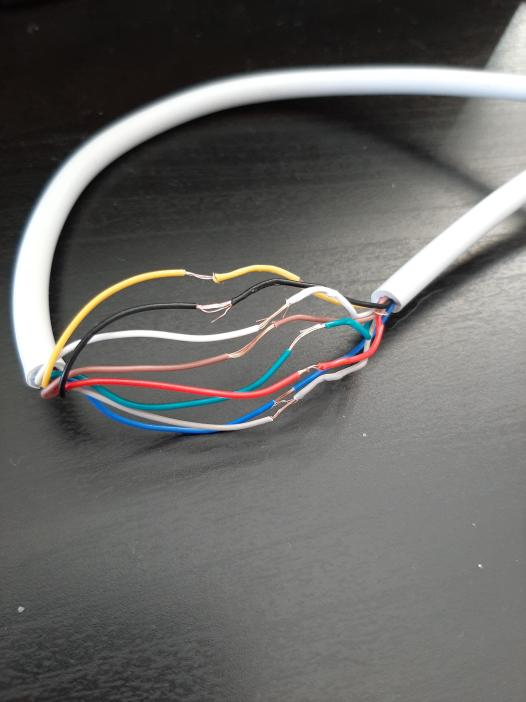
\includegraphics[scale=0.2]{img/cable.jpg}
  \caption{Cabos Utilizados para o Curto Circuito}
\end{figure}

\newpage

\section{Anexo XVII - Variação do Tamanho das Tramas}

\begin{figure}[htbp]
  \centering        
  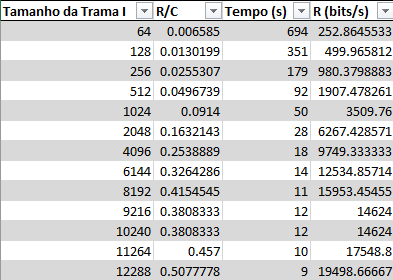
\includegraphics[scale=1]{img/tamanho_da_trama_table.png}
  \caption{Tabela da Variação do Tamanho das Tramas}
\end{figure}

\begin{figure}[htbp]
  \centering        
  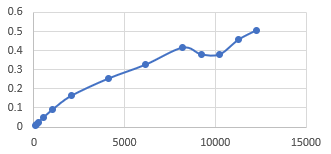
\includegraphics[scale=1]{img/tamanho_da_trama.png}
  \caption{Gráfico da Variação do Tamanho das Tramas}
\end{figure}

\section{Anexo XVIII - Variação da Capacidade de Ligação \textit{Baudrate}}

\begin{figure}[htbp]
  \centering        
  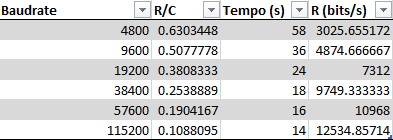
\includegraphics[scale=1]{img/baudrate_table.png}
  \caption{Tabela da Variação da Capacidade de Ligação}
\end{figure}

\begin{figure}[htbp]
  \centering        
  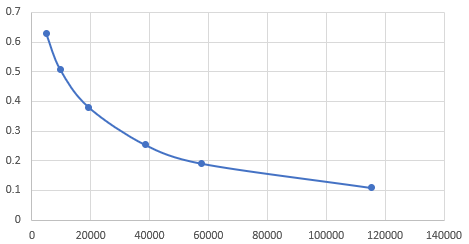
\includegraphics[scale=1]{img/baudrate.png}
  \caption{Gráfico da Variação da Capacidade de Ligação}
\end{figure}

\newpage

\section{Anexo XIX - Geração do Atraso de Propagação}

\begin{figure}[htbp]
  \centering        
  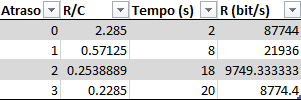
\includegraphics[scale=1]{img/atraso_table.png}
  \caption{Tabela da Geração do Atraso de Propagação}
\end{figure}

\begin{figure}[htbp]
  \centering        
  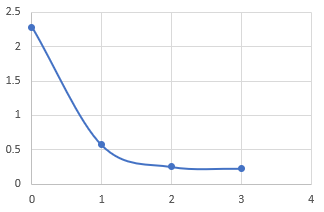
\includegraphics[scale=1]{img/atraso.png}
  \caption{Gráfico da Geração do Atraso de Propagação}
\end{figure}

\section{Anexo XX - Geração Aleatória de Erros}

\begin{figure}[htbp]
  \centering        
  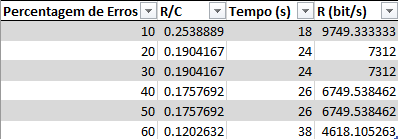
\includegraphics[scale=1]{img/percentagem_table.png}
  \caption{Tabela da Geração Aleatória de Erros}
\end{figure}

\begin{figure}[htbp]
  \centering        
  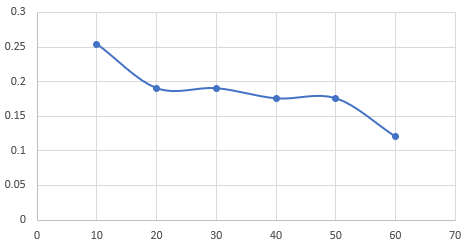
\includegraphics[scale=1]{img/percentagem.png}
  \caption{Gráfico da Geração Aleatória de Erros}
\end{figure}

\end{document}
